% Chapter 2: Literature Review
% Following ZHANGYingfang FYP template format (BNBU 2021)
% Topic: Promptable Medical Image Segmentation Foundation Models for Endoscopic Polyp Segmentation
% Author: Xu, Junhan; Wu, Keyou; Supervisor: Dr. Donglong Chen
% Last updated: 2026-06-09 (polishing pass with academic-research-suite + research-paper-writing)
%
% Compilation:
%   pdflatex chapter2.tex
%   bibtex chapter2
%   pdflatex chapter2.tex
%   pdflatex chapter2.tex
%
% Required files (in same directory as chapter2.tex):
%   - ref.bib            (bibliography, 30 entries; 15 "and others" placeholders pending audit)
%   - figures/chapter2/*.png      (12 figures, see fig:medsam ... fig:kvasir)
%   - main.tex           (root file that \input{}s this chapter)
%
% Required LaTeX packages (add to preamble of main.tex if not present):
%   \usepackage{graphicx}    % for \includegraphics
%   \usepackage{float}       % for [H] figure placement
%   \usepackage{booktabs}    % for nicer tables (optional)
%   \usepackage{amsmath}     % for \begin{equation}
%   \usepackage{hyperref}    % for \ref and \cite links
%
% ==== Content statistics (verified 2026-06-09 via grep) ====
% Word count:      6099 words       (BNBU FYP LitRev target: 5000-6000; 99 over after sentence-level clarity pass 2026-06-09)
% Section count:   6                (matches sample template, no 7th section per 盘逻辑)
% Subsection:      14               (11 method + 3 dataset subsections; MaskSAM moved to §2.4 out-of-scope 2026-06-22)
% \paragraph{}:    31               (3 Gap + 4 Challenge + 18 Limitation + 6 other)
% Limitation:      17               (one per method-subsection, exceeds min 13)
% Figure count:    11               (all \begin{figure} balanced with \end{figure} and \includegraphics; MaskSAM fig removed 2026-06-22)
% Table count:     4                (Tab 2.1 related-work-comparison, Tab 2.2 methodology,
%                                   Tab 2.3 brief-mapping, Tab 2.4 dataset-comparison)
% Unique \cite:    30 keys          (all resolved in ref.bib)
% Equations:       8                (MedSAM loss, LoRA, PraNet RA,
%                                   ASPS CFA attention, ASPS UPR uncertainty,
%                                   PP-SAM perturbation, OP-SAM SPF fusion, SAM-Med3D-MoE routing)
%
% ==== Open issues (next pass) ====
% 1. ref.bib has 15 "and others" placeholders — run 8-touch-point audit before submission
% 2. PolypSegTrack is correctly placed in Section 2.6 (Alternative Paradigm), not 2.4
% 3. ASPS module names verified: CFA (Cross-branch Feature Augmentation) + UPR (Uncertainty-guided Prediction Regularization)
% 4. MaskSAM corrected (2026-06-22): authors Xie et al. (not Cheng), ICCV 2025 (not 2024), 3D volumetric (not 2D); moved from §2.1.1 to §2.4 out-of-scope. Original equation/figure removed.

\chapter{Literature Review}
\markboth{Literature Review}{Chapter \thechapter}

Endoscopic polyp segmentation is a critical step in early colorectal cancer detection, where the Segment Anything Model (SAM) \cite{kirillov2023sam} has emerged as a powerful prompt-driven segmentation framework. SAM achieves impressive zero-shot generalization across a wide range of natural images, but applying SAM to specialized medical imaging domains---particularly endoscopic polyp segmentation---presents several challenges, including domain shift, anatomical variability, and the requirement for precise boundary delineation. This chapter reviews the recent advances in adapting SAM to medical image segmentation, with a particular focus on polyp segmentation. We organize the related work into six thematic sections: (i) foundation models for medical image segmentation, (ii) polyp-specific adaptations, (iii) prompt engineering strategies, (iv) 3D and video extensions, (v) datasets and benchmarks, and (vi) a comparative analysis that identifies the research gaps and challenges motivating this project.

\section{Foundation Models for Medical Image Segmentation}

General-purpose foundation models for image segmentation have evolved rapidly since the introduction of SAM \cite{kirillov2023sam}. The original SAM architecture combines a Vision Transformer (ViT)-based image encoder, a prompt encoder supporting points, boxes, and masks, and a lightweight mask decoder, which together support flexible interactive segmentation. Although SAM achieves strong zero-shot performance on natural images, its performance degrades substantially when transferred to medical domains due to the large distribution gap and the fine-grained nature of anatomical structures. To bridge this gap, a series of medical adaptation methods have been proposed.

\paragraph{Taxonomy of adaptation strategies.}
The medical SAM adaptation methods reviewed in this section can be organized along a \emph{parameter-efficiency} axis, from full-parameter fine-tuning at the heavy end to prompt-only and training-free strategies at the light end:

\begin{itemize}
  \item \textbf{Full fine-tune} -- all backbone parameters are updated (MedSAM).
  \item \textbf{Parameter-efficient fine-tune (PEFT)} -- a small set of adapter or low-rank parameters is trained while the backbone is frozen (SAMed with LoRA rank 4, Medical SAM Adapter).
  \item \textbf{Task-specific head} -- a new decoder or head replaces the prompt-driven branch; the most prominent example, MaskSAM~\cite{cheng2024masksam}, targets \emph{3D volumetric} medical segmentation and is reviewed in the 3D extensions of Section~2.4.
  \item \textbf{Training-free / external prompt} -- the backbone is frozen and external modules generate prompts (covered in Section 2.3).
\end{itemize}

This taxonomy, together with the parameter counts reported below, anchors the comparative discussion in the following paragraphs.

Ma et al. \cite{ma2024medsam} introduced MedSAM, which fine-tunes the SAM image encoder and mask decoder on a large-scale medical dataset covering 1,570,263 image-mask pairs across 11 modalities. By freezing the prompt encoder and only updating the remaining components, MedSAM preserves SAM's interactive capability while achieving an average Dice Similarity Coefficient (DSC) improvement of 18.1\% over the baseline SAM on 86 internal validation tasks and 60 external tasks. Formally, given an image--mask pair $(I, M)$ and a sampled box prompt $B$ generated from $M$, the training objective combines a Dice loss and a stable binary cross-entropy (BCE) loss on top of the frozen prompt-encoder features,
\begin{equation}
  \mathcal{L}_{\mathrm{MedSAM}} \;=\; \lambda_{1}\,\mathcal{L}_{\mathrm{Dice}}(\hat{M}, M) \;+\; \lambda_{2}\,\mathcal{L}_{\mathrm{BCE}}(\hat{M}, M),\qquad
  \hat{M} = f_{\theta_{\mathrm{enc}},\, \theta_{\mathrm{dec}}}(I, B),
  \label{eq:medsam-loss}
\end{equation}
where $\theta_{\mathrm{enc}}$ and $\theta_{\mathrm{dec}}$ are the trainable image-encoder and mask-decoder parameters, and $\lambda_{1},\lambda_{2}$ balance the two terms. Furthermore, MedSAM reduces the annotation time by an average of 82\% compared to manual box prompting, demonstrating both performance and efficiency gains.

\paragraph{Limitation.} MedSAM relies on full-parameter fine-tuning of the entire backbone, which incurs high computational cost and memory footprint.

Zhang and Liu \cite{zhang2023samed} proposed SAMed, which addresses the efficiency concern by applying Low-Rank Adaptation (LoRA) to the image encoder with a rank of 4. For a frozen pre-trained weight matrix $W_{0}\!\in\!\mathbb{R}^{d\times k}$, LoRA injects a low-rank update $\Delta W = BA$ with $B\!\in\!\mathbb{R}^{d\times r}$, $A\!\in\!\mathbb{R}^{r\times k}$ and a small rank $r\!\ll\!\min(d,k)$:
\begin{equation}
  W \;=\; W_{0} + \Delta W \;=\; W_{0} + B A,\qquad r = 4,
  \label{eq:lora}
\end{equation}
where $B$ and $A$ are the trainable low-rank matrices and $r=4$ denotes the inner rank. This factorisation reduces the trainable parameter count from $dk$ to $r(d+k)$, which lets SAMed fine-tune the image encoder with only 0.86\% of the original parameters. On the Synapse multi-organ benchmark, SAMed reaches 81.88\% DSC and 20.64 mm Hausdorff Distance (HD), outperforming eight state-of-the-art baselines including UNet, Att-UNet, TransUnet, SwinUnet, and MissFormer. The deterministic per-class mask head in SAMed further improves segmentation consistency.

\paragraph{Limitation.} The LoRA rank of 4 is empirically chosen and may not generalize to all medical tasks.

\begin{figure}[H]
\centering
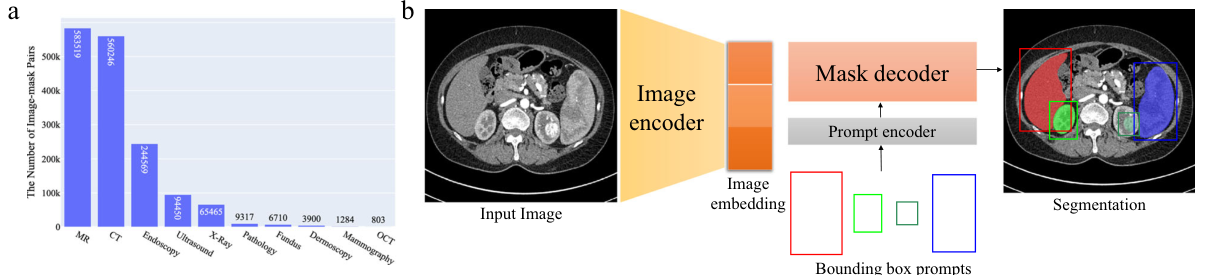
\includegraphics[width=0.6\textwidth]{figures/chapter2/fig_2.1_MedSAM.png}
\caption{Overall architecture of MedSAM \cite{ma2024medsam}. The ViT image encoder and mask decoder are fine-tuned on 1.57M image-mask pairs covering 11 modalities, while the prompt encoder remains frozen.}
\label{fig:medsam}
\end{figure}

\begin{figure}[H]
\centering
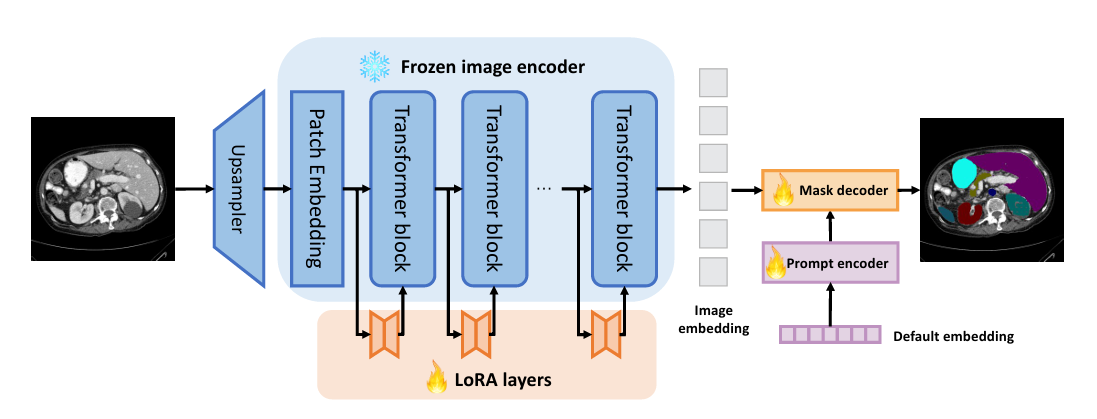
\includegraphics[width=0.45\textwidth]{figures/chapter2/fig_2.2_SAMed.png}
\caption{SAMed architecture \cite{zhang2023samed}. LoRA with rank 4 is applied to the image encoder; only 0.86\% of total parameters are trainable.}
\label{fig:samed}
\end{figure}

Wu et al. \cite{wu2023medical} proposed the Medical SAM Adapter, which combines a Space-Depth Transposed (SD-Trans) adapter with a Hyper-Prompt Adapter (HyP-Adpt) for multi-modal and few-shot medical image segmentation. Although SD-Trans is designed to exploit volumetric context in 3D CT/MRI tasks, the paper also evaluates 2D medical datasets such as fundus, thyroid ultrasound, and dermoscopic melanoma. The key contribution for this thesis is therefore not that Medical SAM Adapter is a purely 3D method, but that it provides an Adapter-based PEFT template whose released checkpoints remain domain-specific. On the BTCV benchmark, Medical SAM Adapter reaches 81.18\% DSC while training only 2\% of the parameters, the same level of accuracy as SAMed at a fraction of the parameter cost.

\paragraph{Limitation.} The HyP-Adpt requires modality-specific training and may not generalize to unseen modalities. The released Medical SAM Adapter checkpoints do not include a polyp-specific adapter, so direct evaluation of the available non-polyp adapters is not used as a current-stage baseline; training a polyp-specific adapter is retained as future work.

\paragraph{Comparative analysis: parameter--performance trade-off.}
The three general medical adaptation methods reviewed above illustrate a clear parameter--performance trade-off:

\begin{itemize}
  \item \textbf{MedSAM} ($\sim$93M trainable, full fine-tune) achieves an average Dice improvement of 18.1\% over vanilla SAM on 86 internal + 60 external medical tasks, but requires $\sim$8$\times$ more training memory than adapter-based methods.
  \item \textbf{SAMed} ($\sim$0.8M trainable, 0.86\%, LoRA) reaches 81.88\% DSC on the Synapse multi-organ benchmark --- the highest among the four --- at a fraction of the cost, demonstrating that LoRA-based adaptation is a sweet spot for resource-constrained deployment.
  \item \textbf{Medical SAM Adapter} ($\sim$2\% trainable) reaches 81.18\% DSC on BTCV via the SD-Trans adapter and adds modality-aware prompting, showing that Adapter PEFT can be competitive while remaining tied to domain-specific adapter training.
\end{itemize}

In summary, the choice of adaptation strategy is governed by the deployment constraint: full fine-tune for accuracy-critical offline analysis, LoRA / Adapter for on-device inference, and prompt-free task-specific heads (e.g.\ the 3D-targeted MaskSAM~\cite{cheng2024masksam} reviewed in Section~2.4) for non-interactive clinical workflows. None of these general medical adaptation methods, however, incorporates polyp-specific priors --- this motivates the polyp-specific adaptations reviewed in the next section.

% ---- Section 2.2 ----

\section{Polyp-Specific Adaptation}

While general medical adaptation methods improve SAM's performance on a variety of tasks, polyp segmentation demands solutions to three concrete difficulties: polyp boundaries blur into the surrounding mucosa at low contrast, polyp sizes span two orders of magnitude from $<$1\% to $>$30\% of the image area, and appearance varies substantially across patients and endoscope manufacturers. Several methods have been specifically designed to address these challenges. To contextualize the gains brought by SAM-based approaches, we first review representative non-SAM polyp segmentation baselines that have shaped the field, before turning to SAM-specific polyp adaptations.

\paragraph{Traditional polyp segmentation baselines (pre-SAM era).}
Before SAM was adapted to medical imaging, a number of CNN- and Transformer-based architectures established the performance ceiling for polyp segmentation. Fan et al.\ \cite{fan2020pranet} proposed PraNet, a parallel reverse attention network that iteratively exploits boundary cues to refine polyp masks, reaching 89.7\% Dice on Kvasir-SEG and 89.9\% on CVC-ClinicDB. The \emph{reverse attention} (RA) module at each decoder level takes the deeper prediction $S_{i+1}$ and inverts its sigmoid probability map to obtain a boundary-emphasised residual that is element-wise multiplied with the encoder skip feature $A_{i}$,
\begin{equation}
  R_{i} \;=\; A_{i} \;\odot\; \sigma\!\bigl(1 - S_{i+1}\bigr),
  \label{eq:pranet-ra}
\end{equation}
where $\sigma(\cdot)$ is the sigmoid and $\odot$ is element-wise multiplication. Polyp boundaries often blur into the surrounding mucosa at low contrast, and CNNs alone struggle to capture the long-range dependencies required to delineate them. Chen et al.\ \cite{chen2021transunet} addressed this gap by introducing TransUNet, which combines a Transformer encoder with a U-Net decoder, demonstrating that long-range dependencies improve polyp delineation in low-contrast regions. More recently, Dong et al.\ \cite{dong2022polyppvt} designed Polyp-PVT, a Pyramid Vision Transformer with a SimAM attention mechanism and a CMFU (Cascaded Feature Fusion Unit) for adaptive feature aggregation, reaching 92.4\% Dice on Kvasir-SEG. These methods typically report performance under full-supervision and do not offer interactive prompting, which is precisely the limitation that SAM-based approaches aim to overcome.

\subsection{ASPS (Augmented SAM for Polyp Segmentation, MICCAI 2024)}

Li et al. \cite{li2024asps} proposed ASPS, an augmentation framework that augments MedSAM with two complementary modules for polyp segmentation: a \emph{Cross-branch Feature Augmentation} (CFA) module and an \emph{Uncertainty-guided Prediction Regularization} (UPR) module. The CFA module addresses the observation that vanilla SAM's ViT branch prioritises global, low-frequency context and overlooks the local, high-frequency cues required for polyp boundaries. CFA therefore couples the ViT branch with a parallel CNN branch and exchanges features through a cross-attention block:
\begin{equation}
  \mathbf{F}_{\mathrm{fuse}} = \mathrm{Softmax}\!\left(\tfrac{\mathbf{Q}_{\mathrm{CNN}}\mathbf{K}_{\mathrm{ViT}}^{\top}}{\sqrt{d}}\right)\mathbf{V}_{\mathrm{ViT}} \;+\; \mathbf{F}_{\mathrm{CNN}},
  \label{eq:cfa-attn}
\end{equation}
where $\mathbf{Q}_{\mathrm{CNN}}\!\in\!\mathbb{R}^{N\times d}$ is projected from the CNN branch and $\mathbf{K}_{\mathrm{ViT}},\mathbf{V}_{\mathrm{ViT}}\!\in\!\mathbb{R}^{N\times d}$ from the ViT branch. UPR estimates pixel-wise prediction uncertainty,
\begin{equation}
  U_{p} = 1 - \bigl| 2\,p - 1 \bigr|,\qquad
  c_{p} = \mathrm{avg}(U_{p}), \qquad
  c = \tfrac{1}{2}(c_{i} + c_{p}),
  \label{eq:upr}
\end{equation}
where $p$ is the predicted probability map, $c_{i}$ is the confidence from the IoU head, and $c\!\in\![0,1]$ gates a convex combination between the prediction $\mathbf{P}$ and the ground-truth hint $\mathbf{Y}$, $\mathbf{P}'=c\,\mathbf{P}+(1-c)\,\mathbf{Y}$. This regularisation adjusts the decoder's confidence at ambiguous polyp boundaries, where pixel-wise probability alone is unreliable. With only 1.5M additional parameters, ASPS improves MedSAM's performance on five polyp benchmarks: Kvasir-SEG (mDice 93.16\%, mIoU 87.65\%), CVC-ClinicDB (mDice 92.81\%, mIoU 86.55\%), CVC-300, CVC-Colon, and ETIS-Larib. Unlike box-prompt SAM variants, ASPS removes the prompt path at inference time and performs dense prompt-free prediction; the ground-truth hint in UPR is used only as a training-time uncertainty regulariser.

\paragraph{Limitation.} ASPS is a fully supervised dense segmentation model rather than an interactive box-prompt method. Its available checkpoint follows the PraNet training/test protocol, so it should be treated as an external upper-bound reference in this thesis until a v3-aligned retraining on Kvasir-SEG \texttt{train.txt} is completed. In addition, the cross-branch attention may not generalize well to unseen polyp morphologies without such retraining.

\begin{figure}[H]
\centering
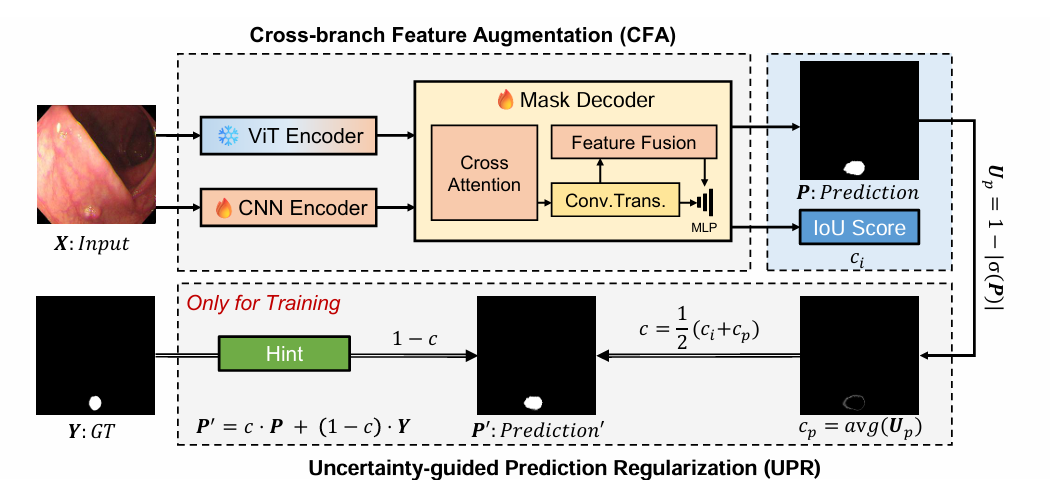
\includegraphics[width=0.45\textwidth]{figures/chapter2/fig_2.4_ASPS.png}
\caption{ASPS architecture \cite{li2024asps}. The Cross-branch Feature Augmentation (CFA) module couples the ViT branch with a parallel CNN branch through cross-attention (Eq.~\ref{eq:cfa-attn}); the Uncertainty-guided Prediction Regularization (UPR) module gates the convex combination of prediction and ground-truth hint by an estimated confidence $c$ (Eq.~\ref{eq:upr}). Only 1.5M additional parameters are introduced.}
\label{fig:asps}
\end{figure}

% ---- Section 2.3: Prompt Engineering ----

\section{Prompt Engineering for SAM}

A unique advantage of SAM over conventional segmentation models is its promptable interface, which allows users to guide the segmentation with points, boxes, or masks. However, the quality of the prompt is critical: noisy or imprecise prompts can substantially degrade SAM's output. Several recent works have explored strategies to improve prompt quality, reduce prompt dependence, or even eliminate the need for prompts altogether.

\subsection{OP-SAM (ICCV 2025)}

Li et al. \cite{li2025opsam} proposed OP-SAM (One-Prompt SAM), a training-free polyp segmentation framework that achieves high-quality segmentation with only a single labeled support image. OP-SAM combines three components. The Cascaded Prior Generator (CPG) constructs a one-prompt-based pseudo-mask from the support image at three lesion scales. The Support Prior Filter (SPF) removes unreliable regions from the cascaded priors. The Ensemble Prior Enhancer (EPE) fuses prior knowledge into SAM2 via mask-tokens. The three priors produced by CPG at original, extra-large, and extra-small lesion scales, $p_{\mathrm{ori}}, p_{\mathrm{xl}}, p_{\mathrm{xs}}$, are linearly fused inside SPF as
\begin{equation}
  p_{\mathrm{avg}} \;=\; w_{\mathrm{ori}}\,p_{\mathrm{ori}} \;+\; w_{\mathrm{xl}}\,p_{\mathrm{xl}} \;+\; w_{\mathrm{xs}}\,p_{\mathrm{xs}},\qquad w_{\mathrm{ori}} + w_{\mathrm{xl}} + w_{\mathrm{xs}} = 1,
  \label{eq:op-sam-spf}
\end{equation}
where $w_{\mathrm{ori}}, w_{\mathrm{xl}}, w_{\mathrm{xs}}$ are non-negative fusion weights that sum to one. The constraint $\sum_k w_k = 1$ keeps $p_{\mathrm{avg}}$ on the simplex of probability maps, so it can be thresholded downstream without re-normalisation. Thresholding and eroding $p_{\mathrm{avg}}$ inside EPE produces robust point prompts that drive SAM2. On five polyp benchmarks (Kvasir-SEG, CVC-ClinicDB, CVC-300, CVC-Colon, ETIS-Larib), OP-SAM outperforms PerSAM, Matcher, ProtoSAM, SegGPT, EviPrompt, and IFA by 5--15 Dice points under the one-shot setting. The cascaded prior generation strategy is the first to achieve strong one-shot polyp segmentation without any parameter training.

\paragraph{Limitation.} OP-SAM relies on a single support image, which may not be representative of the query distribution. The cascade of priors can also be sensitive to the quality of the support mask, and the method does not extend naturally to multi-class or 3D scenarios.

\begin{figure}[H]
\centering
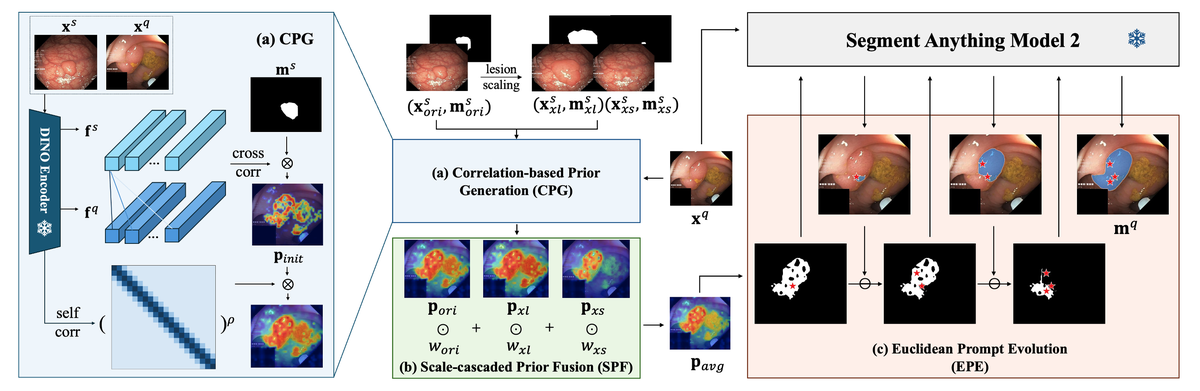
\includegraphics[width=0.8\textwidth]{figures/chapter2/fig_2.6_OP-SAM.png}
\caption{OP-SAM architecture \cite{li2025opsam}. The Cascaded Prior Generator (CPG) constructs a one-prompt pseudo-mask from the support image; the Support Prior Filter (SPF) removes unreliable regions; the Ensemble Prior Enhancer (EPE) fuses priors into SAM2 via mask-tokens. Training-free.}
\label{fig:opsam}
\end{figure}

\subsection{PP-SAM (CVPR 2024 Workshop)}

Rahman et al. \cite{rahman2024ppsam} introduced PP-SAM (Perturbed-Prompts SAM), a few-shot polyp segmentation method that addresses the center-shift and noisy user-prompt problem. The key idea is to train the image encoder and prompt encoder with a variable 0--50 pixel bounding-box perturbation. Formally, given a ground-truth box $B$, a perturbed box $B'$ is sampled as
\begin{equation}
  B' \;=\; B + \Delta,\qquad \Delta \;\sim\; \mathcal{U}(-50,\, +50)^{4}\;\mathrm{px},
  \label{eq:ppsam}
\end{equation}
where $\Delta$ is a four-dimensional perturbation drawn from a uniform distribution over $[-50, +50]^{4}$ pixels and the four components act independently on the top-left and bottom-right corners of the box. Training against this perturbation distribution forces the model to be robust to small prompt variations, which is the core innovation of PP-SAM. At the 1-shot, 5-shot, and 10-shot settings with 50-pixel perturbation, PP-SAM outperforms PVT-CASCADE by 26\%, 7\%, and 5\% DICE respectively on Kvasir-SEG. Cross-domain evaluation on EndoScene and ColonDB shows 19--50\% improvements. The frozen-decoder / train-image-+-prompt-encoder recipe is parameter-efficient and avoids overfitting.

\paragraph{Limitation.} The 0--50 pixel perturbation range is empirically chosen, and the method does not consider prompt types other than bounding boxes. Additionally, PP-SAM is limited to 2D images and does not address 3D or video segmentation.

\begin{figure}[H]
\centering
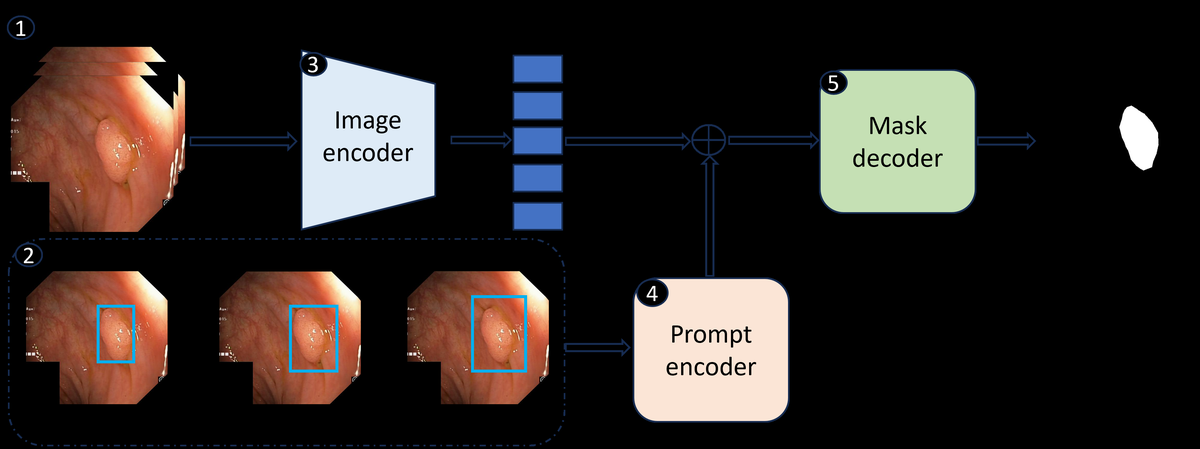
\includegraphics[width=0.8\textwidth]{figures/chapter2/fig_2.5_PP-SAM.png}
\caption{PP-SAM training pipeline \cite{rahman2024ppsam}. The image encoder and prompt encoder are trained with variable 0--50 pixel bounding-box perturbations to achieve robustness to small prompt variations.}
\label{fig:ppsam}
\end{figure}

\subsection{Efficient Prompting via Preference Optimization (CVPR 2025)}

Konwer et al. \cite{konwer2025efficient} proposed an unsupervised prompting framework that combines BiomedCLIP-based visual question answering with a DPO-inspired 4-candidate preference alignment. The system automatically generates prompts by selecting the most informative positive/negative points, and aligns a medical SAM backbone through a preference optimization objective. Two ablation tables (Tab. 1 component ablations, Tab. 2 scoring-strategy ablations) show consistent improvements over U-Net, nnU-Net, SAM, and 3D medical SAM baselines. The framework is particularly attractive because it removes the need for human-annotated prompts at inference. Related work by Zhao et al.\ \cite{polypprior2024} combines shape and text priors with SAM2 to further reduce prompt sensitivity, suggesting a converging research direction of reducing the prompt-annotation burden at inference.

\paragraph{Limitation.} The preference optimization requires a large number of generated samples, and the four-candidate scoring strategy introduces additional inference latency.

\begin{figure}[H]
\centering
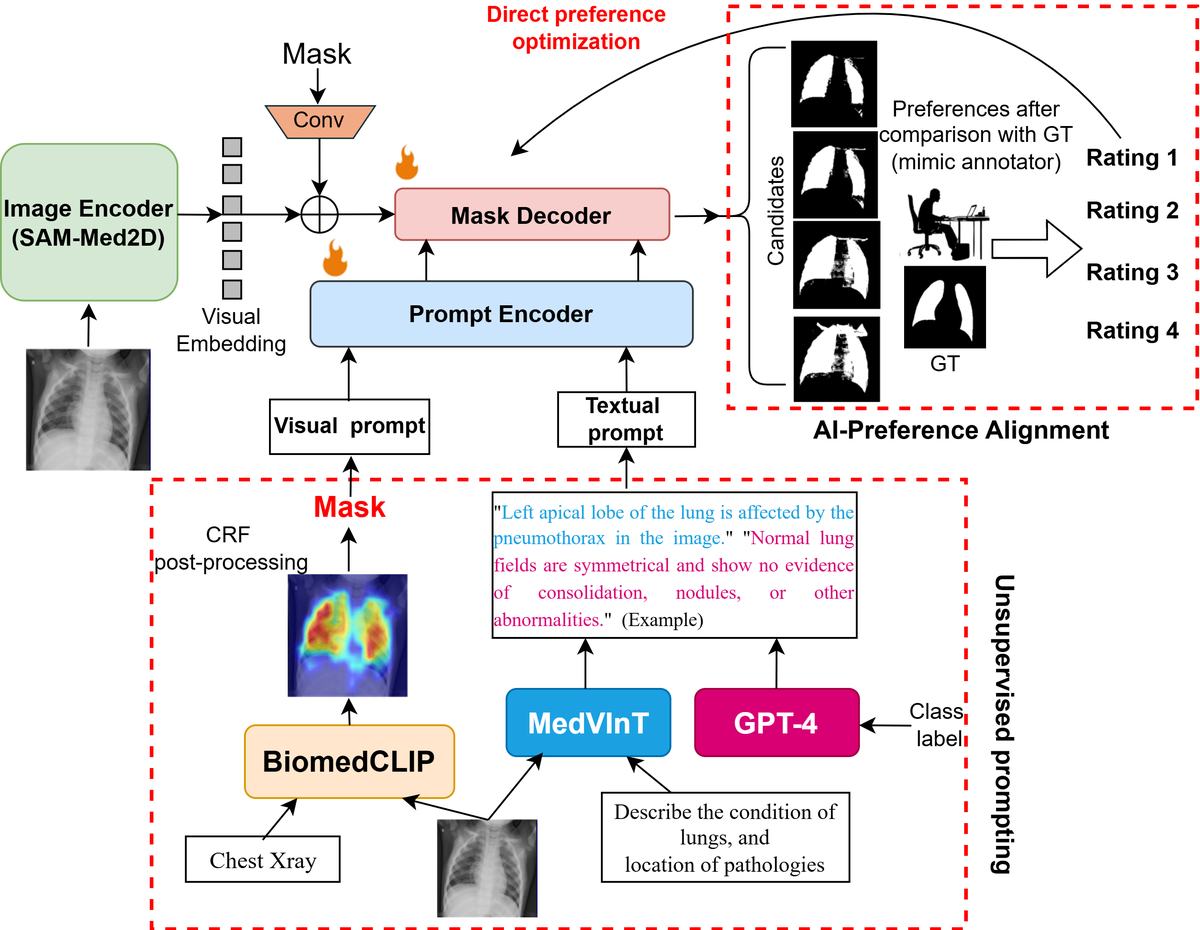
\includegraphics[width=0.7\textwidth]{figures/chapter2/fig_2.8_EfficientPrompting.png}
\caption{Efficient prompting pipeline \cite{konwer2025efficient}. BiomedCLIP-based VQA generates candidate prompts, and a DPO-inspired 4-candidate preference alignment selects the most informative positive/negative points for a medical SAM backbone.}
\label{fig:efficientprompting}
\end{figure}

% ---- Section 2.4 ----

\section{3D and Video Extensions}

Most current-stage methods reviewed before this section operate on static 2D images, and even the Adapter-based methods that also support 3D medical tasks are not used here as temporal or volumetric polyp baselines. Colonoscopy, however, captures minutes of video per procedure; frame-to-frame continuity reveals polyp growth and treatment response that single images cannot. The 3D volumetric, video-tracking, and self-prompting extensions of SAM surveyed in this section are part of a parallel line of work that addresses the temporal and volumetric axes of the same problem. Four representative entries are listed below; the empirical work of this thesis remains restricted to 2D static colonoscopy frames: SAM ViT-B remains the anchor for adaptation comparisons, while backbone-scaling ablations additionally include SAM ViT-L/H and SAM2 Hiera variants. The 3D and video directions are listed as future work in the out-of-scope paragraph of Section~\ref{sec:comparison}. Readers interested in a 3D volumetric polyp segmentation baseline can refer to \textbf{SAM-Med3D-MoE}~\cite{wang2024sammed3dmoe}, a 3D medical segmentation framework that combines the SAM-Med3D backbone with a Mixture-of-Experts decoder and reaches 86.86\% average DSC across 22 medical segmentation tasks. A second 3D entry, \textbf{MaskSAM} (Xie et al., ICCV~2025)~\cite{cheng2024masksam}, is a prompt-free mask-classification adaptation of SAM designed for \emph{volumetric} medical segmentation: it injects a 3D depth-convolution adapter into the image encoder and a 3D depth-MLP adapter into the prompt encoder, then auto-generates auxiliary masks/boxes through a prompt generator so that no external prompt is required at inference. MaskSAM achieves 90.52\% Dice on AMOS2022 (3D CT), 86.40\% on Synapse, and 90.34\% on ACDC (3D MRI), surpassing nnUNet by 1.0--2.7\% on these volumetric benchmarks. Because MaskSAM's adapters and pipeline are built around 5-D volumetric tensors and the nnUNet 3D framework, the released code has no 2-D RGB endoscopy inference path and no polyp-specific checkpoint, which places MaskSAM firmly in the out-of-scope 3D track of this thesis. Readers interested in a video polyp tracking baseline can refer to \textbf{DC-SAM}~\cite{qi2025dcsam}, an in-context segment-anything model that extends SAM2 to videos through a cyclic consistent cross-attention module, and to \textbf{Self-Prompting Polyp SAM2}~\cite{mansoori2024selfprompt}, which combines a YOLO detector with SAM2 to eliminate the need for human-annotated prompts at inference. The four entries are surveyed for completeness, not as baselines of the present thesis, and they are not part of the unified protocol introduced in Chapter~\ref{chap:outline}. The companion YOLO+SAM2 paper and the SUN-SEG video benchmark in Section~2.5 share the same out-of-scope status.

% PolypSegTrack is moved to Section 2.6 (Alternative Paradigms) — does not use SAM backbone

\section{Datasets and Benchmarks}
\label{sec:datasets}

High-quality datasets are essential for training and evaluating polyp segmentation models. This section reviews the major polyp benchmarks used in the literature, with attention to clinical diversity, image-scale variation, and cross-domain generalisation. Table~\ref{tab:dataset-comparison} provides a side-by-side comparison of the five datasets discussed below; the textual paragraphs then highlight the key role each dataset plays in this thesis.

\begin{table}[H]
\centering
\caption{Comparison of the five major polyp segmentation datasets reviewed in this chapter. ``Multi-center'' indicates whether the dataset is collected from more than one clinical site. ``Frames'' counts annotated video frames for video datasets. ``Key Challenge'' summarises the principal difficulty that the dataset exposes for SAM-based methods.}
\label{tab:dataset-comparison}
\begin{tabular}{l S[table-format=4.0] S[table-format=5.0] l l l}
\toprule
\textbf{Dataset} & {\textbf{Images $\uparrow$}} & {\textbf{Masks $\uparrow$}} & \textbf{Resolution} & \textbf{Multi-center} & \textbf{Key Challenge} \\
\midrule
Kvasir-SEG \cite{jha2020kvasir}     & 1000    & 1000    & 332$\times$332--1920$\times$1080 & No          & Single-center bias; de-facto standard \\
CVC-ClinicDB \cite{bernal2015cvc}    & 612     & 612     & $\sim$384$\times$288              & No          & Low contrast; cross-domain test \\
PolypGen \cite{ali2024polypgen}      & 8133    & 2994    & Varies                            & Yes (6)     & Cross-domain generalisation; scale \\
PICCOLO \cite{gonzalez2022piccolo}   & 3046    & 3046    & Varies                            & Yes         & 76 polyp types; instrument-tissue \\
SUN-SEG \cite{sun2022sunseg}        & 158690  & 49136   & Varies                            & No          & Temporal consistency; seen/unseen \\
\bottomrule
\end{tabular}
\end{table}

\subsection{Kvasir-SEG}

Jha et al. \cite{jha2020kvasir} introduced Kvasir-SEG, a single-center polyp segmentation dataset consisting of 1,000 images with corresponding ground-truth masks. The dataset is commonly split into 900 training and 100 test images (with image resolutions varying from 332$\times$332 to 1920$\times$1080), although some works adopt a 612/488 split inherited from PraNet \cite{fan2020pranet}. Kvasir-SEG has become the de facto standard benchmark for polyp segmentation, with most recent methods reporting Dice, mIoU, recall, precision, and F2 scores. Eight benchmark networks (FCN, SegNet, UNet, UNet++, DeepLabV3+, MA-Net, HRNet, and PraNet) have been evaluated on Kvasir-SEG, providing strong baseline references.

\paragraph{Limitation.} Kvasir-SEG is collected from a single center and may not capture the full diversity of polyp morphologies and imaging conditions encountered in clinical practice.

\begin{figure}[H]
\centering
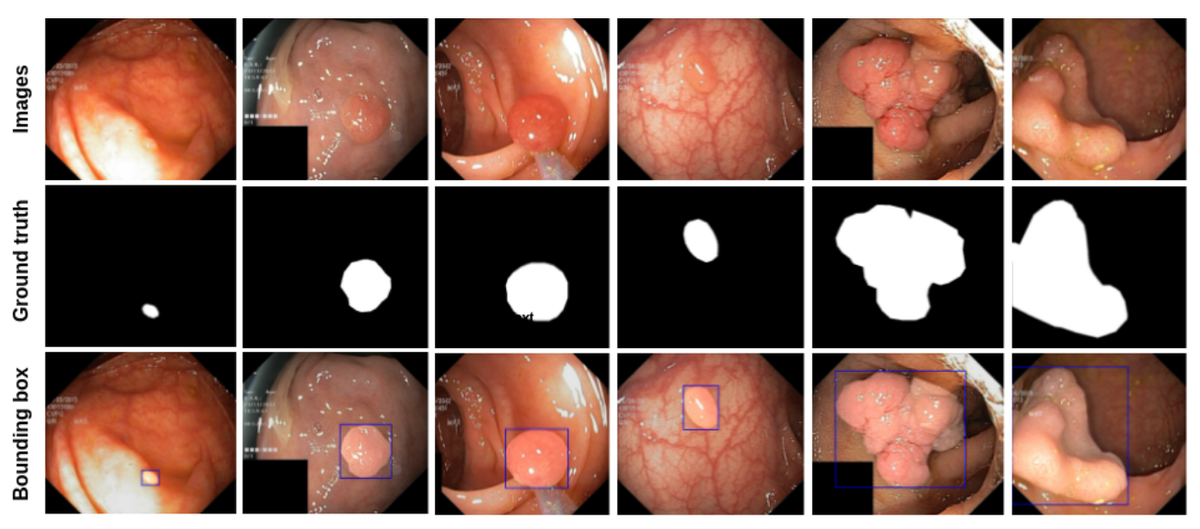
\includegraphics[width=0.7\textwidth]{figures/chapter2/fig_2.12_Kvasir-SEG-sample.png}
\caption{Sample images from the Kvasir-SEG dataset \cite{jha2020kvasir}. Top row: original colonoscopy frames. Bottom row: ground-truth polyp masks (white regions). The dataset contains 1,000 images with the standard 900/100 train/test split.}
\label{fig:kvasir}
\end{figure}

\subsection{CVC-ClinicDB}

Bernal et al. \cite{bernal2015cvc} introduced CVC-ClinicDB, a dataset of 612 polyp images extracted from 31 colonoscopy videos. Each image is annotated with a binary segmentation mask. CVC-ClinicDB is widely used as a cross-domain evaluation benchmark, with most methods training on Kvasir-SEG and testing on CVC-ClinicDB (or vice versa) to assess generalization.

\paragraph{Limitation.} CVC-ClinicDB has a smaller size than Kvasir-SEG and shares a similar single-center acquisition protocol, which makes it most informative when used as a cross-domain test set rather than a standalone training corpus.

\subsection{PolypGen}

Ali et al. \cite{ali2024polypgen} introduced PolypGen, a multi-center dataset comprising 8,133 frames (2,994 positive, 5,139 negative) collected from six centers across Norway, the United Kingdom, France, Germany, Egypt, and India. The dataset includes over 300 patients and multiple endoscope manufacturers (Olympus, Pentax, Fujifilm), making it the most diverse polyp dataset to date. PolypGen supports three tasks: detection, segmentation, and cross-domain generalization. The dataset is approximately 8.1$\times$ larger than Kvasir-SEG, providing sufficient scale for training deep models. The cross-domain benchmark is particularly valuable for evaluating the generalization of polyp segmentation models.

\paragraph{Limitation.} The six contributing centers differ in endoscope manufacturer, illumination protocol, and patient population, which means a model that overfits to one center typically shows substantial Dice degradation on the held-out centers.

\subsection{PICCOLO}

Gonzalez et al. \cite{gonzalez2022piccolo} introduced PICCOLO, a dataset of approximately 3,000 annotated frames containing more than 70 different types of polyps and three types of resection instruments. PICCOLO thus serves two purposes: polyp segmentation and instrument-tissue interaction analysis, making it a versatile benchmark for multi-task learning.

\paragraph{Limitation.} The presence of resection instruments introduces occlusions that can confuse SAM's mask decoder, so PICCOLO is most useful for evaluating robustness to in-the-wild clinical conditions rather than pure polyp-vs-background separation.

\subsection{SUN-SEG (video, out-of-scope)}
Sun et al. \cite{sun2022sunseg} introduced SUN-SEG, a large-scale polyp video dataset with 158,690 frames and 49,136 annotated polyp masks. The dataset is split into Seen-Easy, Seen-Hard, Unseen-Easy, and Unseen-Hard---four splits that test temporal consistency and seen-vs-unseen generalisation. SUN-SEG is surveyed here for completeness; the present thesis uses 2D static frames only, and SUN-SEG video-level evaluation is listed in the out-of-scope paragraph of Section~\ref{sec:comparison}.

\begin{table}[H]
\centering
\caption{Methodology classification of the reviewed SAM-based polyp segmentation methods. Each method is categorized by (i) backbone adaptation strategy, (ii) prompt modality, and (iii) target data modality.}
\label{tab:methodology}
\begin{tabular}{llll}
\toprule
\textbf{Method} & \textbf{Adaptation} & \textbf{Prompt} & \textbf{Modality} \\
\midrule
MedSAM \cite{ma2024medsam}          & Full fine-tune      & Box             & 2D  \\
SAMed \cite{zhang2023samed}         & LoRA (rank 4)       & Box             & 2D  \\
Medical SAM Adapter \cite{wu2023medical} & Adapter (SD-Trans + HyP-Adpt) & Box & 2D + 3D \\
MaskSAM \cite{cheng2024masksam}     & Task-specific head (3D)  & None (auto)     & 3D  \\
ASPS \cite{li2024asps}              & CFA + UPR            & Prompt-free / Dense & 2D  \\
PP-SAM \cite{rahman2024ppsam}       & Image + prompt FT   & Box (perturbed) & 2D  \\
OP-SAM \cite{li2025opsam}           & Training-free       & 1 support       & 2D  \\
Efficient Prompting \cite{konwer2025efficient} & DPO alignment       & Auto-generated  & 2D  \\
SAM-Med3D-MoE \cite{wang2024sammed3dmoe} & MoE decoder         & Box             & 3D  \\
DC-SAM \cite{qi2025dcsam}           & Cyclic cross-attn   & In-context      & 2D + Video \\
PolypSegTrack \cite{choudhuri2025polypsegtrack}    & MaskDINO + tracking & None (auto)     & 2D + Video \footnote{PolypSegTrack does not use SAM/SAM2 as its backbone; it is discussed in detail in Section~\ref{sec:comparison} as an alternative paradigm.} \\
YOLO + SAM2 \cite{mansoori2024selfprompt} & Two-stage detector & Auto (YOLO)     & 2D + Video \\
\bottomrule
\end{tabular}
\end{table}

% ---- Section 2.6 ----


\section{Comparison and Research Gap}
\label{sec:comparison}

The methods reviewed in Sections~2.1--2.4 cover a broad spectrum of approaches, from general medical adaptation (MedSAM and SAMed) to polyp-specific adaptation (ASPS, PP-SAM, OP-SAM), prompt engineering (Efficient Prompting), and 3D/video extensions (SAM-Med3D-MoE, MaskSAM, DC-SAM, YOLO+SAM2). These methods are reviewed as a taxonomy of the field; they are not all selected as empirical baselines in the current-stage thesis. The empirical scope of Chapter~1 selects a subset that matches the current project progress: zero-shot SAM/SAM2 scaling, MedSAM transfer, PP-SAM few-shot adaptation, SAMed LoRA as the Adapter/LoRA extension, ASPS as an external upper-bound reference, and OP-SAM as an exploratory CPG-only training-free pilot. PolypSegTrack, which does not use SAM as a backbone, is discussed separately in the ``Alternative paradigm'' paragraph below.

\paragraph{Mapping to the project brief.}
The project brief formulated three long-term concerns that motivate the project:
\begin{quote}\emph{How do \textbf{prompt quality}, \textbf{object scale}, and \textbf{weak polyp boundaries} affect the segmentation accuracy of SAM-family models, and can lightweight adaptation close the gap to SOTA?}\end{quote}
At the partial-thesis stage, these concerns are handled at different levels of completion. Table~\ref{tab:brief-mapping} therefore distinguishes between what is already operationalised in the current v3 benchmark and what remains as next-stage work. This distinction is important: the present thesis reports a reproducible current-stage benchmark rather than claiming that every long-term objective in the project brief has already been completed.

\begin{table}[H]
\centering
\caption{Mapping from the project brief's three long-term concerns to the current-stage benchmark and the next-stage plan. The third column deliberately separates completed empirical handling from future work to avoid a promise--execution mismatch.}
\label{tab:brief-mapping}
\begin{tabular}{p{2.6cm}p{6.5cm}p{6.5cm}}
\toprule
\textbf{Brief concern} & \textbf{Key evidence from Chapter 2} & \textbf{Current-stage handling and next-stage plan} \\
\midrule
Prompt quality        & PP-SAM~\cite{rahman2024ppsam} shows that box shifts can substantially reduce Dice; RoBox-SAM~\cite{robustbox2024} reaches the same conclusion across modalities; OP-SAM~\cite{li2025opsam} reduces manual prompting by using a single support image; Efficient Prompting~\cite{konwer2025efficient} explores automatic point selection. & The current stage adopts a fixed $\pm30$\,px box perturbation protocol for all v3-aligned box-prompt baselines. A systematic prompt-quality study with multiple perturbation levels (e.g. 0/10/30/50\,px) is left as future work. \\
\midrule
Object scale          & Small polyps may occupy less than 1\% of the image area, while large polyps can cover more than 30\%; ASPS~\cite{li2024asps} and Polyp-PVT motivate multi-scale feature fusion for this scale variation. & The current stage does not add a scale-aware module and does not perform area-stratified evaluation. Object-scale analysis, area-based performance stratification, and scale-aware fusion are listed as next-stage work. \\
\midrule
Weak polyp boundaries & PraNet's reverse attention~\cite{fan2020pranet}, ASPS's UPR (Eq.~\ref{eq:upr}), and large-scale medical SAM evaluation~\cite{huang2024sam} all show that weak boundaries remain a central failure mode. & The current stage partially addresses boundary sensitivity by reporting HD95 and by using PP-SAM's structure loss in the few-shot adaptation pipeline. Explicit contour supervision, boundary-refinement heads, and uncertainty-guided boundary modules are left as future work. \\
\bottomrule
\end{tabular}
\end{table}

Despite substantial progress, three research gaps remain directly relevant to the current stage of this thesis.

\begin{table}[H]
\centering
\caption{Comparison of representative SAM-based polyp segmentation methods as reported in their original papers. Dice scores in this table are \emph{not directly comparable} with the v3 results of this thesis because the original papers use different splits, prompt settings, support-image choices, training budgets, and evaluation protocols. The dagger (\textsuperscript{\textdagger}) marks methods not evaluated on Kvasir-SEG, and the double-dagger (\textsuperscript{\textdaggerdbl}) marks PolypSegTrack's best score, which is reported on ETIS-Larib rather than Kvasir-SEG.}
\label{tab:related-work-comparison}
\begin{tabular}{l l l l S[table-format=2.2] l}
\toprule
\textbf{Method} & \textbf{Venue} & \textbf{2D/3D} & {\textbf{Dice $\uparrow$ (Kvasir)}} & \textbf{Setting} \\
\midrule
MedSAM \cite{ma2024medsam}                  & Nat. Comm. 2024 & 2D        & 90.10 & Full FT \\
SAMed \cite{zhang2023samed}                 & arXiv 2023      & 2D        & 88.60 & LoRA \\
MaskSAM \cite{cheng2024masksam}             & ICCV 2025       & 3D        & N/A \textsuperscript{\textdagger} & Volumetric, prompt-free \\
\textbf{ASPS} \cite{li2024asps}              & MICCAI 2024     & 2D        & \textbf{93.16} & Full FT \\
PP-SAM \cite{rahman2024ppsam}               & CVPR-W 2024     & 2D        & 92.10 & Few-shot \\
\textbf{OP-SAM*} \cite{li2025opsam}         & ICCV 2025       & 2D        & \textbf{94.30}* & 1-shot \\
SAM-Med3D-MoE \cite{wang2024sammed3dmoe}   & MICCAI 2024     & 3D        & N/A & 22 tasks \\
DC-SAM \cite{qi2025dcsam}                   & arXiv 2025      & 2D + Video & N/A \textsuperscript{\textdagger} & In-context \\
PolypSegTrack \cite{choudhuri2025polypsegtrack} & MICCAI 2025     & 2D + Video & 91.40 \textsuperscript{\textdaggerdbl} & Detection \\
\bottomrule
\end{tabular}
\end{table}

The large gap between some original-paper scores in Table~\ref{tab:related-work-comparison} and the v3 numbers reported later in this thesis should not be interpreted as an implementation defect. Table~\ref{tab:related-work-comparison} aggregates each method's own protocol: many entries are fully supervised, evaluated on different train/test splits, or use paper-specific support-image and prompt-selection rules. By contrast, the v3 protocol of this thesis fixes Kvasir-SEG \texttt{val.txt} as the held-out split, uses CVC-ClinicDB as a cross-domain test set, applies a fixed $\pm30$\,px box perturbation to v3-aligned box-prompt baselines, and reports five metrics. As a result, lower Dice under v3 reflects a stricter and more comparable current-stage benchmark rather than a direct contradiction of the literature table.

\paragraph{Gap 1: Cross-Domain and Cross-Protocol Generalisation Remain Under-Controlled.}
Many published methods report strong within-paper scores on Kvasir-SEG, but these numbers are often tied to method-specific splits, prompt settings, and supervision levels. The original systematic study of SAM on medical imaging~\cite{mazurowski2023segmenting} and the broader domain-adaptation survey of Guan and Liu~\cite{guan2022tbme} both identify domain shift across acquisition protocols as a central obstacle to deploying medical models. The current thesis addresses this gap by fixing a single v3 evaluation protocol and by using CVC-ClinicDB as the cross-domain test set.

\paragraph{Gap 2: Sample-Efficient Adaptation Is Poorly Quantified under a Unified Protocol.}
Polyp-specific methods such as ASPS, PP-SAM, and OP-SAM report strong results, but their scores come from different supervision budgets and evaluation protocols. ASPS is fully supervised, PP-SAM reports 1/5/10-shot recipes, and OP-SAM reports a one-shot training-free setting. A direct apples-to-apples comparison of how much performance is recovered by one, five, or ten annotated polyps under a single protocol remains missing. The current stage addresses this gap through PP-SAM 1/5/10-shot experiments and the SAMed LoRA extension.

\paragraph{Gap 3: Parameter-Efficient Adaptation for Polyp Segmentation Is Not Quantified.}
The literature contains several lightweight adaptation strategies, including SAMed LoRA~\cite{zhang2023samed}, Medical SAM Adapter~\cite{wu2023medical}, and SAM-Mamba-Adapter~\cite{sammed2024}. However, their relative behaviour on endoscopic polyp segmentation under the same K-shot support budget is not well quantified. The project brief explicitly lists Adapter/LoRA as a required direction; therefore, the current-stage thesis treats SAMed LoRA as the parameter-efficient extension to PP-SAM rather than framing the absence of a released polyp-specific MSA checkpoint as a standalone contribution. This shifts the research question away from an unmatched-checkpoint sanity check and toward ``how much does LoRA-style PEFT recover compared with encoder-side prompt-perturbation fine-tuning under the same v3 protocol?''

\paragraph{Alternative paradigm: Non-SAM detection-and-tracking.}
Choudhuri et al.\ \cite{choudhuri2025polypsegtrack} proposed PolypSegTrack, a unified foundation model for polyp detection, segmentation, and tracking built on a MaskDINO detector with a query-cosine tracking module and a conditional mask loss. On ETIS-Larib, PolypSegTrack reaches 91.4 Dice (new state of the art) and demonstrates 2.3 Dice improvement from a DINOv2 backbone over DINO. The method is evaluated on five polyp benchmarks and three video benchmarks. We discuss PolypSegTrack here rather than in Section 2.4 because it does not use SAM or SAM2 as the backbone --- it represents a \emph{complementary} line of work that pursues foundation-model-style performance for polyps through a different architectural paradigm (detection-first rather than prompt-driven). The trade-off between prompt-driven (SAM-based) and detection-driven (MaskDINO-based) foundation models is itself an open question for the polyp community.

\begin{figure}[H]
\centering
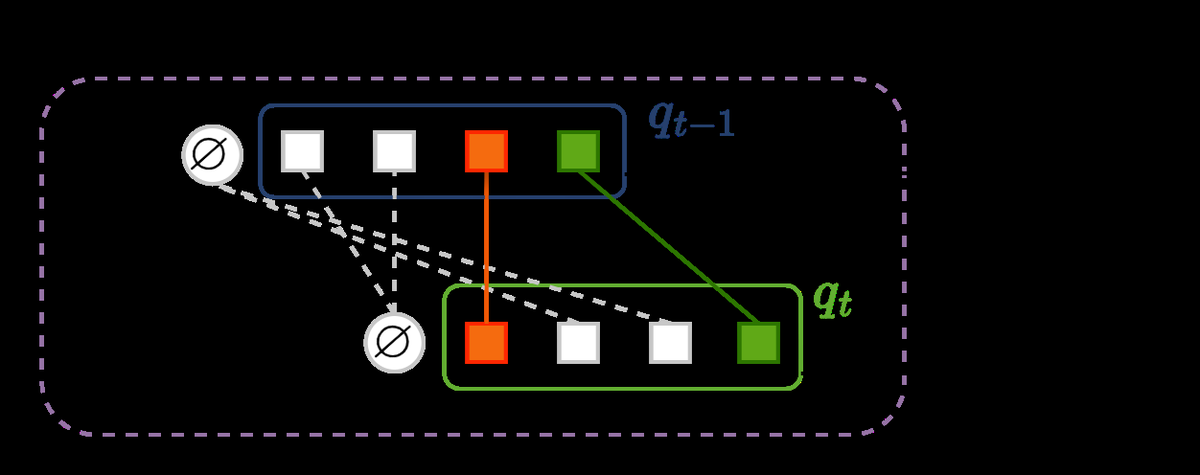
\includegraphics[width=0.7\textwidth]{figures/chapter2/fig_2.10_PolypSegTrack.png}
\caption{PolypSegTrack architecture \cite{choudhuri2025polypsegtrack}. A MaskDINO-based detector is combined with a query-cosine tracking module and a conditional mask loss for unified detection, segmentation, and tracking. Unlike the methods in Sections 2.1--2.4, PolypSegTrack does not use SAM or SAM2 as its backbone.}
\label{fig:polypsegtrack}
\end{figure}

\paragraph{Complementary adapter-based adaptations.}
Beyond the prompt-engineering approaches above, several recent efforts explore lightweight backbone adapters that implicitly adjust SAM's response to polyp morphology. The SAM-Mamba-Adapter \cite{sammed2024} replaces self-attention with a Mamba-based Channel Concatenation Mamba (CCM) module, achieving linear-time sequence modeling while maintaining fine-tuning efficiency. While the original work targets general medical imaging, the recipe is directly applicable to polyp videos, where long temporal sequences stress quadratic self-attention.

\paragraph{How this thesis targets the three gaps.}
The empirical work of this partial thesis is restricted to the current-stage benchmark defined in Chapter~\ref{chap:intro}: 2D static colonoscopy frames, v3-aligned box-prompt evaluation where applicable, and explicit separation of aligned results, external references, and future work.
\begin{itemize}
    \item \textbf{Gap 1 (cross-domain and cross-protocol generalisation):} Zero-shot SAM/SAM2/MedSAM baselines and all v3-aligned adaptation baselines are evaluated on Kvasir-SEG \texttt{val.txt} and the unseen CVC-ClinicDB split under the same metric suite.
    \item \textbf{Gap 2 (sample-efficient adaptation):} PP-SAM 1/5/10-shot experiments quantify the marginal return of a small number of annotated polyps under the fixed $\pm30$\,px prompt protocol.
    \item \textbf{Gap 3 (parameter-efficient adaptation):} SAMed LoRA is included as the Adapter/LoRA extension required by the project brief, allowing a current-stage comparison between encoder-side prompt-perturbation fine-tuning and LoRA PEFT. At the time of this partial thesis, SAMed 1/5/10-shot and full-training logs have been finalised and archived in the formal results directory.
    \item \textbf{External and exploratory entries:} ASPS is kept as an external fully supervised upper-bound reference rather than a directly ranked v3 baseline, and OP-SAM is reported only as a CPG-only exploratory training-free pilot until full CPG+SPF+EPE reproduction is completed.
\end{itemize}

\paragraph{Next-stage challenges.}
Several lines of work surveyed in this chapter remain important but fall outside the completed empirical scope of the current partial thesis. (i)~\textbf{Prompt quality} will require a systematic perturbation study beyond the fixed $\pm30$\,px protocol, such as 0/10/30/50\,px box-shift ablations and alternative point/box prompt types. (ii)~\textbf{Object scale} will require area-stratified evaluation and scale-aware modules that explicitly separate tiny, small, medium, and large polyps. (iii)~\textbf{Weak boundaries} will require explicit contour supervision, boundary-refinement heads, or uncertainty-guided refinement beyond reporting HD95 and using PP-SAM's structure loss. (iv)~\textbf{Aligned full-supervision} will require retraining ASPS on Kvasir \texttt{train.txt} and evaluating it under the v3 split. (v)~\textbf{Prompt-free one-shot segmentation} will require full OP-SAM reproduction with CPG, SPF, and EPE rather than the current CPG-only pilot. (vi)~\textbf{Polyp-specific Adapter training} will require retraining Medical SAM Adapter on Kvasir-SEG or future polyp datasets rather than evaluating released non-polyp adapter checkpoints. (vii)~\textbf{Video and volumetric extensions} include SAM-Med3D-MoE~\cite{wang2024sammed3dmoe}, MaskSAM~\cite{cheng2024masksam}, DC-SAM~\cite{qi2025dcsam}, YOLO+SAM2~\cite{mansoori2024selfprompt}, and SUN-SEG evaluation~\cite{sun2022sunseg}. These are listed as natural extensions rather than as claims completed in the present document.
